\section{Arquitectura de Simulación del Workspace ROS2}

El workspace \texttt{phantom\_ws} constituye el entorno de desarrollo basado en ROS2 para el manipulador PhantomX Pincher. Este espacio de trabajo proporciona una infraestructura completa de simulación que integra descripción del robot, planificación de movimiento mediante MoveIt2, y visualización en tiempo real con RViz. La arquitectura permite transiciones fluidas entre operación en simulación y control de hardware real, facilitando flujos de trabajo de desarrollo, pruebas y despliegue.

%==============================================================================
\subsection{Introducción al Entorno de Simulación}
%==============================================================================

El workspace \texttt{phantom\_ws} implementa un stack completo de simulación que incluye los siguientes componentes:

\begin{itemize}
    \item Descripción del robot y modelos 3D mediante URDF/SDF
    \item Capacidades de planificación de movimiento a través de MoveIt2
    \item Visualización en tiempo real con RViz
    \item Múltiples modos de simulación (controladores simulados, Gazebo, hardware real)
    \item Interfaces de comando de alto nivel para control del robot
\end{itemize}

La arquitectura modular del workspace separa claramente las responsabilidades entre paquetes especializados, siguiendo las mejores prácticas de ROS2 y facilitando el mantenimiento y extensión del sistema.

%==============================================================================
\subsection{Estructura del Workspace}
%==============================================================================

El workspace sigue la estructura estándar de ROS2 con un directorio \texttt{src/} que contiene todos los paquetes, junto con directorios \texttt{build/}, \texttt{install/} y \texttt{log/} generados durante el proceso de compilación.

\subsubsection{Organización de Directorios}

\begin{minted}[fontsize=\footnotesize, breaklines, frame=single]{text}
phantom_ws/
|-- src/
|   |-- phantomx_pincher/                    # Metapaquete
|   |-- phantomx_pincher_description/        # Modelos URDF/SDF
|   |-- phantomx_pincher_moveit_config/      # Configuracion MoveIt
|   |-- phantomx_pincher_bringup/            # Archivos launch
|   |-- phantomx_pincher_commander_cpp/      # Interfaz comando C++
|   |-- phantomx_pincher_demos/              # Scripts demo y mundos
|   |-- phantomx_pincher_opencv/             # Soporte camara/vision
|   |-- phantomx_pincher_interfaces/         # Mensajes personalizados
|   +-- pincher_control/                     # Control hardware real
|-- build/                                   # Artefactos compilacion
|-- install/                                 # Paquetes instalados
+-- log/                                     # Registros compilacion
\end{minted}

\subsubsection{Resumen de Paquetes}

La Tabla \ref{tab:paquetes_workspace} presenta una descripción general de todos los paquetes del workspace y sus funciones principales.

\begin{table}[H]
\centering
\caption{Paquetes del workspace y sus propósitos}
\label{tab:paquetes_workspace}
\small
\begin{tabular}{|p{5.5cm}|p{9cm}|}
\hline
\textbf{Paquete} & \textbf{Propósito} \\
\hline
\texttt{phantomx\_pincher} & Metapaquete que agrupa descripción y configuración MoveIt \\
\texttt{phantomx\_pincher\_description} & Modelos URDF/SDF, mallas 3D y configuraciones de visualización \\
\texttt{phantomx\_pincher\_moveit\_config} & Configuración completa de MoveIt2 para planificación de movimiento \\
\texttt{phantomx\_pincher\_bringup} & Punto de entrada principal para simulación y control de hardware \\
\texttt{phantomx\_pincher\_commander\_cpp} & Interfaz de comando de alto nivel en C++ \\
\texttt{phantomx\_pincher\_demos} & Scripts de demostración y mundos de Gazebo \\
\texttt{phantomx\_pincher\_opencv} & Integración de sensor de cámara \\
\texttt{phantomx\_pincher\_interfaces} & Definiciones de mensajes ROS2 personalizados \\
\texttt{pincher\_control} & Interfaz de servomotores Dynamixel para hardware real \\
\hline
\end{tabular}
\end{table}

%==============================================================================
\subsection{Descripción Detallada de Paquetes}
%==============================================================================

\subsubsection{phantomx\_pincher\_description}

Este paquete contiene la definición completa del modelo del robot utilizando URDF (Unified Robot Description Format) con macros Xacro para modularidad. El paquete incluye:

\begin{itemize}
    \item \textbf{Xacros URDF}: Archivos modulares de descripción del robot
    \begin{itemize}
        \item \texttt{phantomx\_pincher.urdf.xacro} -- Punto de entrada principal URDF
        \item \texttt{phantomx\_pincher\_arm.xacro} -- Definiciones de articulaciones/eslabones del brazo
        \item \texttt{phantomx\_pincher\_hardware.xacro} -- Definiciones de interfaz de hardware
        \item \texttt{phantomx\_pincher\_inertial.xacro} -- Propiedades inerciales
    \end{itemize}
    \item \textbf{Mallas 3D}: Mallas STL para colisiones y mallas DAE para visualización
    \item \textbf{Configuración}: Posiciones iniciales de articulaciones y configuraciones de RViz
\end{itemize}

El URDF soporta múltiples parámetros de configuración a través de argumentos Xacro:

\begin{minted}[fontsize=\footnotesize, breaklines, frame=single]{xml}
<!-- Parametros de configuracion del robot -->
<xacro:arg name="ros2_control" default="true"/>
<xacro:arg name="ros2_control_plugin" default="fake"/>
<xacro:arg name="ros2_control_command_interface" default="position"/>
<xacro:arg name="collision" default="true"/>
<xacro:arg name="mimic_finger_joints" default="false"/>
\end{minted}

\subsubsection{phantomx\_pincher\_moveit\_config}

Este paquete proporciona la configuración completa de MoveIt2 para planificación de movimiento. Los componentes clave incluyen:

\paragraph{Configuración SRDF}

El formato SRDF (Semantic Robot Description Format) define:

\begin{itemize}
    \item \textbf{Grupos de Planificación}:
    \begin{itemize}
        \item \texttt{arm} -- Cadena cinemática de 4-DOF desde base hasta efector final
        \item \texttt{gripper} -- Gripper de 2-DOF con articulaciones de dedos
    \end{itemize}
    \item \textbf{Estados Predefinidos}: Configuraciones nombradas como \texttt{up}, \texttt{rest}, \texttt{ready\_near}, \texttt{open}, \texttt{closed}
    \item \textbf{Pares de Colisión}: Verificación de colisión deshabilitada entre eslabones adyacentes
\end{itemize}

\paragraph{Archivos de Configuración}

\begin{itemize}
    \item \texttt{kinematics.yaml} -- Configuración del solver de cinemática inversa KDL
    \item \texttt{joint\_limits.yaml} -- Límites de velocidad y aceleración
    \item \texttt{ompl\_planning.yaml} -- Configuraciones de planificadores OMPL (RRTstar, BiRRT, etc.)
    \item \texttt{controllers\_position.yaml} -- Configuración de controlador de trayectoria de articulaciones
    \item \texttt{servo.yaml} -- Parámetros de MoveIt Servo para control en tiempo real
\end{itemize}

\subsubsection{phantomx\_pincher\_bringup}

El paquete bringup sirve como punto de entrada principal para lanzar la simulación. Proporciona un archivo launch unificado que soporta tanto modos de simulación como de hardware real mediante un único argumento.

\begin{minted}[fontsize=\footnotesize, breaklines, frame=single]{bash}
# Modo simulacion (predeterminado)
ros2 launch phantomx_pincher_bringup phantomx_pincher.launch.py

# Modo hardware real
ros2 launch phantomx_pincher_bringup phantomx_pincher.launch.py \
    use_real_robot:=true
\end{minted}

\paragraph{Argumentos de Launch}

El archivo launch principal acepta los siguientes argumentos:

\begin{itemize}
    \item \texttt{use\_real\_robot} -- Activa control de hardware real (default: \texttt{false})
    \item \texttt{use\_rviz} -- Lanza visualización RViz (default: \texttt{true})
    \item \texttt{rviz\_config} -- Archivo de configuración RViz personalizado
    \item \texttt{use\_gazebo} -- Lanza simulación Gazebo (default: \texttt{false})
    \item \texttt{world} -- Archivo de mundo Gazebo a cargar
\end{itemize}

\subsubsection{phantomx\_pincher\_commander\_cpp}

Este paquete proporciona una interfaz de comando de alto nivel implementada en C++ que simplifica el control del robot mediante MoveIt2. La interfaz expone métodos para:

\begin{itemize}
    \item Comandos de objetivo de articulación (joint goal)
    \item Comandos de objetivo de pose cartesiana (pose goal)
    \item Ejecución de trayectorias planificadas
    \item Control del gripper (apertura/cierre)
    \item Consulta de estado actual del robot
\end{itemize}

\subsubsection{Modos de Hardware Soportados}

La Tabla \ref{tab:modos_hardware} resume los tres modos de hardware soportados por el workspace.

\begin{table}[H]
\centering
\caption{Modos de hardware soportados}
\label{tab:modos_hardware}
\small
\begin{tabular}{|l|p{11cm}|}
\hline
\textbf{Modo} & \textbf{Descripción} \\
\hline
\texttt{fake} & Hardware simulado para pruebas sin física \\
\texttt{ign} & Integración con Ignition Gazebo para simulación con física \\
\texttt{real} & Interfaz real de servomotores Dynamixel \\
\hline
\end{tabular}
\end{table}

%==============================================================================
\subsection{Sistema de Launch y Bringup}
%==============================================================================

El paquete bringup orquesta el lanzamiento de todos los componentes de simulación a través de un sistema jerárquico de archivos launch.

\subsubsection{Archivo Launch Principal}

El archivo \texttt{phantomx\_pincher.launch.py} en el paquete bringup sirve como punto de entrada principal. Lanza condicionalmente diferentes configuraciones de nodos basándose en el argumento \texttt{use\_real\_robot}.

\paragraph{Modo Simulación (use\_real\_robot=false)}

En modo simulación, se lanzan los siguientes nodos:

\begin{enumerate}
    \item \textbf{robot\_state\_publisher}: Publica el árbol TF basado en estados de articulaciones
    \item \textbf{ros2\_control\_node}: Gestor de controladores con plugin de hardware simulado
    \item \textbf{Spawners de Controladores}:
    \begin{itemize}
        \item \texttt{joint\_state\_broadcaster} -- Publica estados de articulaciones
        \item \texttt{joint\_trajectory\_controller} -- Control de trayectoria del brazo
        \item \texttt{gripper\_trajectory\_controller} -- Control del gripper
    \end{itemize}
    \item \textbf{move\_group}: Planificación y ejecución de MoveIt2
    \item \textbf{commander}: Interfaz de comando de alto nivel
    \item \textbf{RViz}: Visualización
\end{enumerate}

\paragraph{Modo Hardware Real (use\_real\_robot=true)}

En modo hardware real, el nodo ros2\_control se reemplaza por la interfaz personalizada de Dynamixel:

\begin{enumerate}
    \item \textbf{robot\_state\_publisher}: Publicación TF
    \item \textbf{follow\_joint\_trajectory\_node}: Interfaz de servomotores Dynamixel
    \item \textbf{move\_group}: Planificación MoveIt2
    \item \textbf{commander}: Interfaz de comando
    \item \textbf{RViz}: Visualización
\end{enumerate}

\subsubsection{Flujo de Control}

La Figura \ref{fig:flujo_control_sim} ilustra el flujo de control en modo simulación.

\begin{figure}[H]
\centering
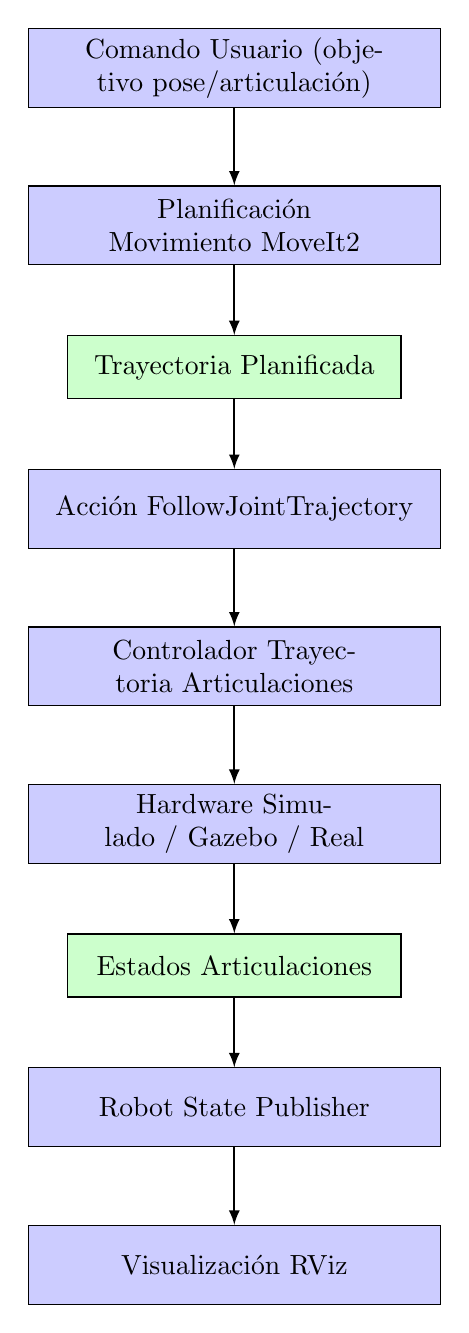
\begin{tikzpicture}[node distance=1.5cm, auto]
    % Estilos
    \tikzstyle{process} = [rectangle, draw, fill=blue!20, text width=5cm, text centered, minimum height=1cm]
    \tikzstyle{data} = [rectangle, draw, fill=green!20, text width=4cm, text centered, minimum height=0.8cm]
    \tikzstyle{arrow} = [thick,-latex]

    % Nodos
    \node (cmd) [process] {Comando Usuario (objetivo pose/articulación)};
    \node (moveit) [process, below of=cmd, yshift=-0.5cm] {Planificación Movimiento MoveIt2};
    \node (traj) [data, below of=moveit, yshift=-0.3cm] {Trayectoria Planificada};
    \node (action) [process, below of=traj, yshift=-0.3cm] {Acción FollowJointTrajectory};
    \node (ctrl) [process, below of=action, yshift=-0.5cm] {Controlador Trayectoria Articulaciones};
    \node (hw) [process, below of=ctrl, yshift=-0.5cm] {Hardware Simulado / Gazebo / Real};
    \node (js) [data, below of=hw, yshift=-0.3cm] {Estados Articulaciones};
    \node (rsp) [process, below of=js, yshift=-0.3cm] {Robot State Publisher};
    \node (rviz) [process, below of=rsp, yshift=-0.5cm] {Visualización RViz};

    % Flechas
    \draw [arrow] (cmd) -- (moveit);
    \draw [arrow] (moveit) -- (traj);
    \draw [arrow] (traj) -- (action);
    \draw [arrow] (action) -- (ctrl);
    \draw [arrow] (ctrl) -- (hw);
    \draw [arrow] (hw) -- (js);
    \draw [arrow] (js) -- (rsp);
    \draw [arrow] (rsp) -- (rviz);
\end{tikzpicture}
\caption{Flujo de control de la simulación. El usuario envía comandos de alto nivel (objetivos de pose o articulación) que MoveIt2 planifica en trayectorias. Estas trayectorias se ejecutan mediante controladores que envían comandos al hardware (simulado o real), cuyos estados se publican de vuelta al sistema para visualización en RViz.}
\label{fig:flujo_control_sim}
\end{figure}

%==============================================================================
\subsection{Configuración de Controladores}
%==============================================================================

Los controladores de trayectoria de articulaciones se configuran en el archivo \texttt{controllers\_position.yaml}:

\begin{minted}[fontsize=\footnotesize, breaklines, frame=single]{yaml}
controller_manager:
  ros__parameters:
    update_rate: 250  # Hz

joint_trajectory_controller:
  ros__parameters:
    joints:
      - phantomx_pincher_arm_shoulder_pan_joint
      - phantomx_pincher_arm_shoulder_lift_joint
      - phantomx_pincher_arm_elbow_flex_joint
      - phantomx_pincher_arm_wrist_flex_joint
    command_interfaces:
      - position
    state_interfaces:
      - position
      - velocity

gripper_trajectory_controller:
  ros__parameters:
    joints:
      - phantomx_pincher_gripper_finger1_joint
      - phantomx_pincher_gripper_finger2_joint
    command_interfaces:
      - position
\end{minted}

\paragraph{Parámetros Clave de Controladores}

\begin{itemize}
    \item \textbf{update\_rate}: Frecuencia de actualización del gestor de controladores (250 Hz)
    \item \textbf{joints}: Lista de articulaciones controladas por cada controlador
    \item \textbf{command\_interfaces}: Tipo de comando enviado a las articulaciones (posición)
    \item \textbf{state\_interfaces}: Información de estado recibida de las articulaciones (posición y velocidad)
\end{itemize}

%==============================================================================
\subsection{Ejecución de la Simulación}
%==============================================================================

\subsubsection{Lanzamiento Básico de Simulación}

Para iniciar la simulación con controladores simulados y RViz:

\begin{minted}[fontsize=\footnotesize, breaklines, frame=single]{bash}
# Compilar el workspace
cd phantom_ws
colcon build --symlink-install

# Cargar el workspace
source install/setup.bash

# Lanzar la simulacion
ros2 launch phantomx_pincher_bringup phantomx_pincher.launch.py
\end{minted}

\subsubsection{Visualización del Modelo del Robot}

Para visualización simple del URDF sin MoveIt:

\begin{minted}[fontsize=\footnotesize, breaklines, frame=single]{bash}
ros2 launch phantomx_pincher_description view.launch.py
\end{minted}

\subsubsection{Ejecución de Demostraciones}

Demostraciones de ejemplo están disponibles en el paquete demos:

\begin{minted}[fontsize=\footnotesize, breaklines, frame=single]{bash}
# Ejecutar ejemplo de objetivo de articulacion
ros2 run phantomx_pincher_demos ex_joint_goal.py

# Ejecutar ejemplo de objetivo de pose
ros2 run phantomx_pincher_demos ex_pose_goal.py

# Ejecutar demo pick and place
ros2 run phantomx_pincher_demos demo_pick_and_place.py
\end{minted}

%==============================================================================
\subsection{Sistemas de Coordenadas}
%==============================================================================

El robot utiliza la siguiente jerarquía de marcos de referencia TF:

\begin{minted}[fontsize=\footnotesize, breaklines, frame=single]{text}
world
+-- base_link
    +-- arm_base_link
        +-- arm_shoulder_pan_link      (Articulacion 1)
            +-- arm_shoulder_lift_link (Articulacion 2)
                +-- arm_elbow_flex_link    (Articulacion 3)
                    +-- arm_wrist_flex_link    (Articulacion 4)
                        +-- gripper_finger_base_link
                            +-- gripper_finger1_link
                            +-- gripper_finger2_link
                            +-- end_effector
\end{minted}

El marco \texttt{end\_effector} es el punto de referencia para comandos de pose cartesiana y se ubica en el centro de los dedos del gripper.

\paragraph{Transformaciones de Coordenadas}

El sistema ROS2 mantiene automáticamente las transformaciones entre todos los marcos mediante el árbol TF. Esto permite:

\begin{itemize}
    \item Conversión automática entre coordenadas de diferentes marcos
    \item Consulta de pose del efector final en cualquier marco de referencia
    \item Planificación de movimiento en espacio cartesiano
    \item Detección de colisiones en espacio 3D
\end{itemize}

%==============================================================================
\subsection{Integración con MoveIt2}
%==============================================================================

MoveIt2 proporciona las capacidades de planificación de movimiento del sistema. La integración incluye:

\subsubsection{Planificadores Disponibles}

El workspace está configurado con múltiples algoritmos de planificación de OMPL (Open Motion Planning Library):

\begin{itemize}
    \item \textbf{RRTConnect}: Planificador rápido basado en muestreo
    \item \textbf{RRTstar}: Versión óptima asintóticamente de RRT
    \item \textbf{PRM}: Roadmap probabilístico para múltiples consultas
    \item \textbf{BiRRT}: RRT bidireccional
    \item \textbf{LBKPIECE}: Planificador basado en descomposición del espacio
\end{itemize}

\subsubsection{Servicios de Planificación}

MoveIt2 expone los siguientes servicios para planificación:

\begin{itemize}
    \item \texttt{/plan\_kinematic\_path}: Planifica trayectoria entre estados
    \item \texttt{/compute\_ik}: Calcula cinemática inversa para pose objetivo
    \item \texttt{/compute\_fk}: Calcula cinemática directa para configuración de articulaciones
    \item \texttt{/get\_planning\_scene}: Obtiene representación actual del entorno
\end{itemize}

%==============================================================================
\subsection{Conclusión del Sistema de Simulación}
%==============================================================================

El workspace \texttt{phantom\_ws} proporciona un entorno completo de simulación para el manipulador PhantomX Pincher. La arquitectura modular, construida sobre ROS2, MoveIt2 y RViz, habilita:

\begin{itemize}
    \item Prototipado rápido y pruebas en simulación
    \item Transición fluida a hardware real
    \item Planificación de movimiento flexible con múltiples algoritmos
    \item Visualización y depuración en tiempo real
    \item Interfaces de comando de alto nivel para desarrollo de aplicaciones
\end{itemize}

La separación de responsabilidades entre paquetes (descripción, configuración, bringup, control) sigue las mejores prácticas de ROS2 y facilita el mantenimiento y extensión del sistema. Esta infraestructura de simulación constituye la base para el desarrollo de algoritmos de clasificación de objetos mediante visión por computador y control autónomo del manipulador en el kit educativo.